% mnras_guide.tex
%
% MNRAS LaTeX user guide
%
% v3.0 released 22 May 2015
% (version numbers match those of mnras.cls)
%
% Copyright (C) Royal Astronomical Society 2015
% Authors:
% Keith T. Smith (Royal Astronomical Society)

% Change log
%
% v3.0   September 2013 - May 2015
%    First version: complete rewrite of the user guide
%    Basic structure taken from mnras_template.tex by the same author

%%%%%%%%%%%%%%%%%%%%%%%%%%%%%%%%%%%%%%%%%%%%%%%%%%
% Basic setup. Most papers should leave these options alone.
\documentclass[a4paper,fleqn,usenatbib]{mnras}

%%%%% AUTHORS - PLACE YOUR OWN PACKAGES HERE %%%%%

% MNRAS is set in Times font. If you don't have this installed (most LaTeX
% installations will be fine) or prefer the old Computer Modern fonts, comment
% out the following line
\usepackage{newtxtext,newtxmath}
% Depending on your LaTeX fonts installation, you might get better results with one of these:
%\usepackage{mathptmx}
%\usepackage{txfonts}

% Use vector fonts, so it zooms properly in on-screen viewing software
% Don't change these lines unless you know what you are doing
\usepackage[T1]{fontenc}
\usepackage{ae,aecompl}


%%%%% AUTHORS - PLACE YOUR OWN PACKAGES HERE %%%%%

% Only include extra packages if you really need them. Common packages are:
\usepackage{graphicx}	% Including figure files
\usepackage{amsmath}	% Advanced maths commands
\usepackage{amssymb}	% Extra maths symbols
\usepackage{hyperref}

%%%%%%%%%%%%%%%%%%%%%%%%%%%%%%%%%%%%%%%%%%%%%%%%%%

%%%%%% AUTHORS - PLACE YOUR OWN MACROS HERE %%%%%%

% Please keep new commands to a minimum, and use \newcommand not \def to avoid
% overwriting existing commands. Example:
%\newcommand{\pcm}{\,cm$^{-2}$}	% per cm-squared
\newcommand{\kms}{\,km\,s$^{-1}$} % kilometres per second
\newcommand{\bibtex}{\textsc{Bib}\!\TeX} % bibtex. Not quite the correct typesetting, but close enough

%%%%%%%%%%%%%%%%%%%%%%%%%%%%%%%%%%%%%%%%%%%%%%%%%%


% Use vector fonts, so it zooms properly in on-screen viewing software
% Don't change these lines unless you know what you are doing
\usepackage[T1]{fontenc}
\usepackage{ae,aecompl}

% MNRAS is set in Times font. If you don't have this installed (most LaTeX
% installations will be fine) or prefer the old Computer Modern fonts, comment
% out the following line
\usepackage{newtxtext,newtxmath}
% Depending on your LaTeX fonts installation, you might get better results with one of these:
%\usepackage{mathptmx}
%\usepackage{txfonts}

%%%%%%%%%%%%%%%%%%% TITLE PAGE %%%%%%%%%%%%%%%%%%%

% Title of the paper, and the short title which is used in the headers.
% Keep the title short and informative.
\title[Magritte]{Magritte: a new Multidimensional Accelerated General-purpose Radiative Transfer code}

% The list of authors, and the short list which is used in the headers.
% If you need two or more lines of authors, add an extra line using \newauthor
\author[F. De Ceuster]{ F. De Ceuster$^{1,2}$\thanks{Contact e-mail: \href{frederik.deceuster@kuleuven.be}{frederik.deceuster@kuleuven.be}}, J. Yates$^{1}$, J. Hetherington$^{3}$, P.A. Boyle$^{4}$, L. Decin$^{2}$, S. Viti$^{1}$ and T.G. Bisbas$^{5,6}$
\\ \\
% List of institutions
$^{1}$Department of Physics and Astronomy, University College London, Gower Place, London, WC1E 6BT, UK \\
$^{2}$Department of Physics and Astronomy, Institute of Astronomy, KU Leuven, Celestijnenlaan 200D, 3001 Leuven, Belgium \\
$^{3}$Research Software Development Group, University College London, Podium Building, 1 Eversholt Street, London, NW12DN, UK \\
$^{4}$School of Physics and Astronomy, The University of Edinburgh, Edinburgh EH9 3FD, UK \\
$^{5}$Department of Astronomy and Physics, University of Florida, Gainesville, FL 32611, USA \\
$^{6}$Max-Planck-Institut f\"ur Extraterrestrische Physik, Giessenbachstrasse 1, D-85748 Garching, Germany}


% These dates will be filled out by the publisher
\date{Last updated 2011 May 22; in original form 2013 September 5}

% Enter the current year, for the copyright statements etc.
\pubyear{2018}

% Don't change these lines
\begin{document}
\label{firstpage}
\pagerange{\pageref{firstpage}--\pageref{lastpage}}
\maketitle

% Abstract of the paper
\begin{abstract}
The  In this paper we present the basis for a new multidimensional accelerated general-purpose radiative transfer code, called Magritte.
\end{abstract}

% Select between one and six entries from the list of approved keywords.
% Don't make up new ones.
\begin{keywords}
radiative transfer, astrochemistry, methods: numerical
\end{keywords}

%%%%%%%%%%%%%%%%%%%%%%%%%%%%%%%%%%%%%%%%%%%%%%%%%%

%%%%%%%%%%%%%%%%% BODY OF PAPER %%%%%%%%%%%%%%%%%%

% The MNRAS class isn't designed to include a table of contents, but for this document one is useful.
% I therefore have to do some kludging to make it work without masses of blank space.
\begingroup
\let\clearpage\relax
% \tableofcontents
\endgroup
\newpage


\section{Introduction}

The Radiative Transfer problem is one of the oldest and

New C++ code based on 3D-PDR \citet{Bisbas2012} improved performance. separate modules for chemistry, radiative transfer and thermal balance.

The paper is organized as follows. In section \ref{CompSc} we present the new computational scheme and the different modules of Magritte. Section \ref{Benchmarks} describes the different benchmarks that were done to test the code and to compare its performance with 3D-PDR. In Section \ref{Applications} we present the new applications that have become feasible through the nove Finally our conclusions are discussed in Section \ref{Conclusions}.


\section{Computational Scheme}
\label{CompSc}

Although Magritte is based on 3D-PDR, the whole code has been rewritten from scratch.


\begin{figure}
	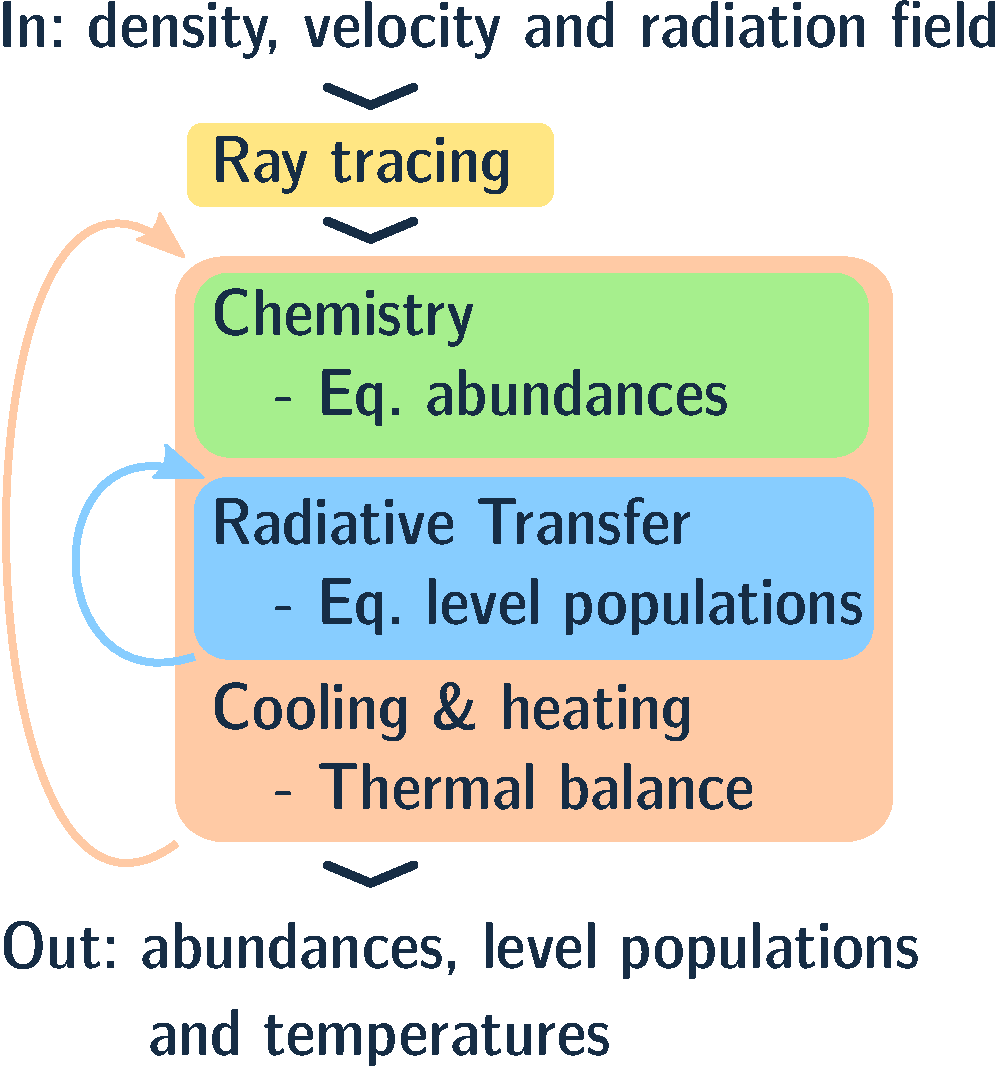
\includegraphics[width=\columnwidth]{figures/scheme.pdf}
  \caption{Scheme of the Magritte workflow, different boxes represent the different modules.}
  \label{scheme}
\end{figure}



\subsection{Data structures and memory layout}

Magritte assumes an unstructured grid of cells


Much better memory scaling and impoved overall performance.

Plot of memory use as function of the number of grid cells, Magritte vs. 3D-PDR.


\subsection{Modules}

To facilitate the incorporation of Magritte in other codes, the code is structerd into separate dedicated modules each handling a specific part of the calculaltion.

\subsubsection{Ray-tracing}

On the length and time scales considered in Magritte simulations, light travels on straight lines. The first step in

The direction of a ray is determined by the HEALPix\footnote{\href{http://healpix.sourceforge.net}{healpix.sourceforge.net}} discretization of the sphere \citet{Gorski2005}

\subsubsection{Chemistry}

Magritte determines the relative abundances of a limited number of atomic and molecular species at each cell. This is done by solving the time-dependent chemistry of a self-contained network of formation and destruction reactions. The chemical network is a subset of the most recent UMIST data base of reaction rates \citet{Woodall2007}, consisting of 320 reactions between 33 species (including electrons), and includes photoionization and photodissociation reactions in addition to the standard gas-phase chemistry.

\subsubsection{Radiative transfer}

Lines plus continuum.

The line data were taken from the Leiden Atomic and Molecular Database \citep[LAMDA,][]{Schoier2005}.

Acceleration methods Ng-acceleration \citet{Ng1974} and Rybicki-Hummer acceleration scheme \citet{Rybicki1991}. The combination of both acceleration schemes yield a significant speed up in the convergence of the level populations.

Later versions will be able to treat multiple dust scattering

\subsubsection{Thermal balance}

Magritte can self-consitently determine the temperature assuming local thermal balance, i.e. equal heating and cooling rates for each cell. (Argument on time scales?)


\subsection{Parallelization strategy}

\section{Benchmarks}
\label{Benchmarks}



\section{Applications}
\label{Applications}
The modular character of Magritte allows it to be easily used in various astrophysical simulations.


\section{Conclusions}
\label{Conclusions}
We have presented Magritte: a new multidimensional accelerated general-purpose radiative transfer code.

\bigskip

Once all modules are finished and extensively tested, the source code for Magritte and its separate modules will be made freely available on \href{https://github.com/Magritte-code}{github.com/Magritte-code}.


\section*{Acknowledgements}
FDC is supported by the EPSRC iCASE studentship programme, Intel Corporation and Cray Inc.


\bibliography{library}
\bibliographystyle{mnras}


%%%%%%%%%%%%%%%%%%%%%%%%%%%%%%%%%%%%%%%%%%%%%%%%%%


% Don't change these lines
\bsp	% typesetting comment
\label{lastpage}
\end{document}
